\documentclass{article}
\usepackage[utf8]{inputenc}
\usepackage[a4paper, margin=1cm]{geometry}
\usepackage{ifthen}
\usepackage{tikz}
\usepackage{amsmath}
\usepackage{flowchart}
\usetikzlibrary{shapes.geometric, shapes.multipart, arrows, positioning, calc, shadows, backgrounds}
\usepackage{textgreek}
\usepackage{hyperref}
\usepackage{paralist}
\usepackage{tikz-uml}

\tikzstyle{note} = [text width=3cm, 
				fill=black!10,
				align=flush left]
\tikzstyle{base} = [text height=0.5cm,
				minimum width=3cm, 
				minimum height=1.25cm, 
				text centered, 
				text width=3cm, 
				draw=black]
\tikzstyle{ext-resource} = [isosceles triangle,
					draw=black, 
					fill=yellow!20]
\tikzstyle{ext-storage} = [storage,
					minimum width=3cm, 
					minimum height=1.25cm, 
					draw=black, 
					fill=yellow!20]
\tikzstyle{resource} = [base, rectangle, 
				rounded corners,
				 fill=blue!20]
\tikzstyle{timer} = [resource, label={[below]90: \textbf{Timer}}]
\tikzstyle{bucket} = [base, storage, 
			      label={[below]90: \textbf{S3}}, 
			      fill=blue!20]
\tikzstyle{lambda} = [base, 
				rectangle, 
				label={[below]90: {\textbf{\textlambda}}}, 
				fill=orange!20]
\tikzstyle{timed-lambda} = [base,
				rectangle,
				label={[below]90: {\textbf{Timed \textlambda}}}, 
				fill=orange!35]				
%\tikzstyle{io} = [trapezium, trapezium left angle=70, trapezium right angle=110, minimum width=3cm, minimum height=1cm, text centered, draw=black, fill=blue!30]
%\tikzstyle{decision} = [diamond, minimum width=3cm, minimum height=1cm, text centered, draw=black, fill=green!30]
\tikzstyle{arrow} = [thick,>=stealth]
\tikzstyle{trigger} = [thick, >=open triangle 45, green]
\tikzstyle{sync} = [thick,>=triangle 45]
\tikzstyle{async} = [thick,>=open triangle 45]

\newcommand{\returncall}[5]{
	\ifthenelse{\equal{#5}{vertical}}{
		\draw [sync, ->, transform canvas={xshift=-0.5em}] (#1) -- node[anchor=east] {#3} (#2);
		\draw [sync, <-, transform canvas={xshift=0.5em}] (#1) -- node[anchor=west] {#4}(#2);
	}{
		\draw [sync, ->, transform canvas={yshift=0.5em}] (#1) -- node[anchor=south] {#3} (#2);
		\draw [sync, <-, transform canvas={yshift=-0.5em}] (#1) -- node[anchor=north] {#4}(#2);
	}
}

\newcommand{\handshake}[5]{
	\ifthenelse{\equal{#5}{vertical}}{
		\draw [sync, ->, transform canvas={xshift=-0.5em}] (#1) -- node[anchor=east] {#3} (#2);
		\draw [sync, <-, transform canvas={xshift=0.5em}, dashed] (#1) -- node[anchor=west] {#4}(#2);
	}{
		\draw [sync, ->, transform canvas={yshift=0.5em}] (#1) -- node[anchor=south] {#3} (#2);
		\draw [sync, <-, transform canvas={yshift=-0.5em}, dashed] (#1) -- node[anchor=north] {#4}(#2);
	}
}


\renewcommand{\emph}[1]{\textbf{#1}}

\begin{document}
\thispagestyle{empty}

\section{Interview transfer service}\begin{center}
\begin{figure}[h]
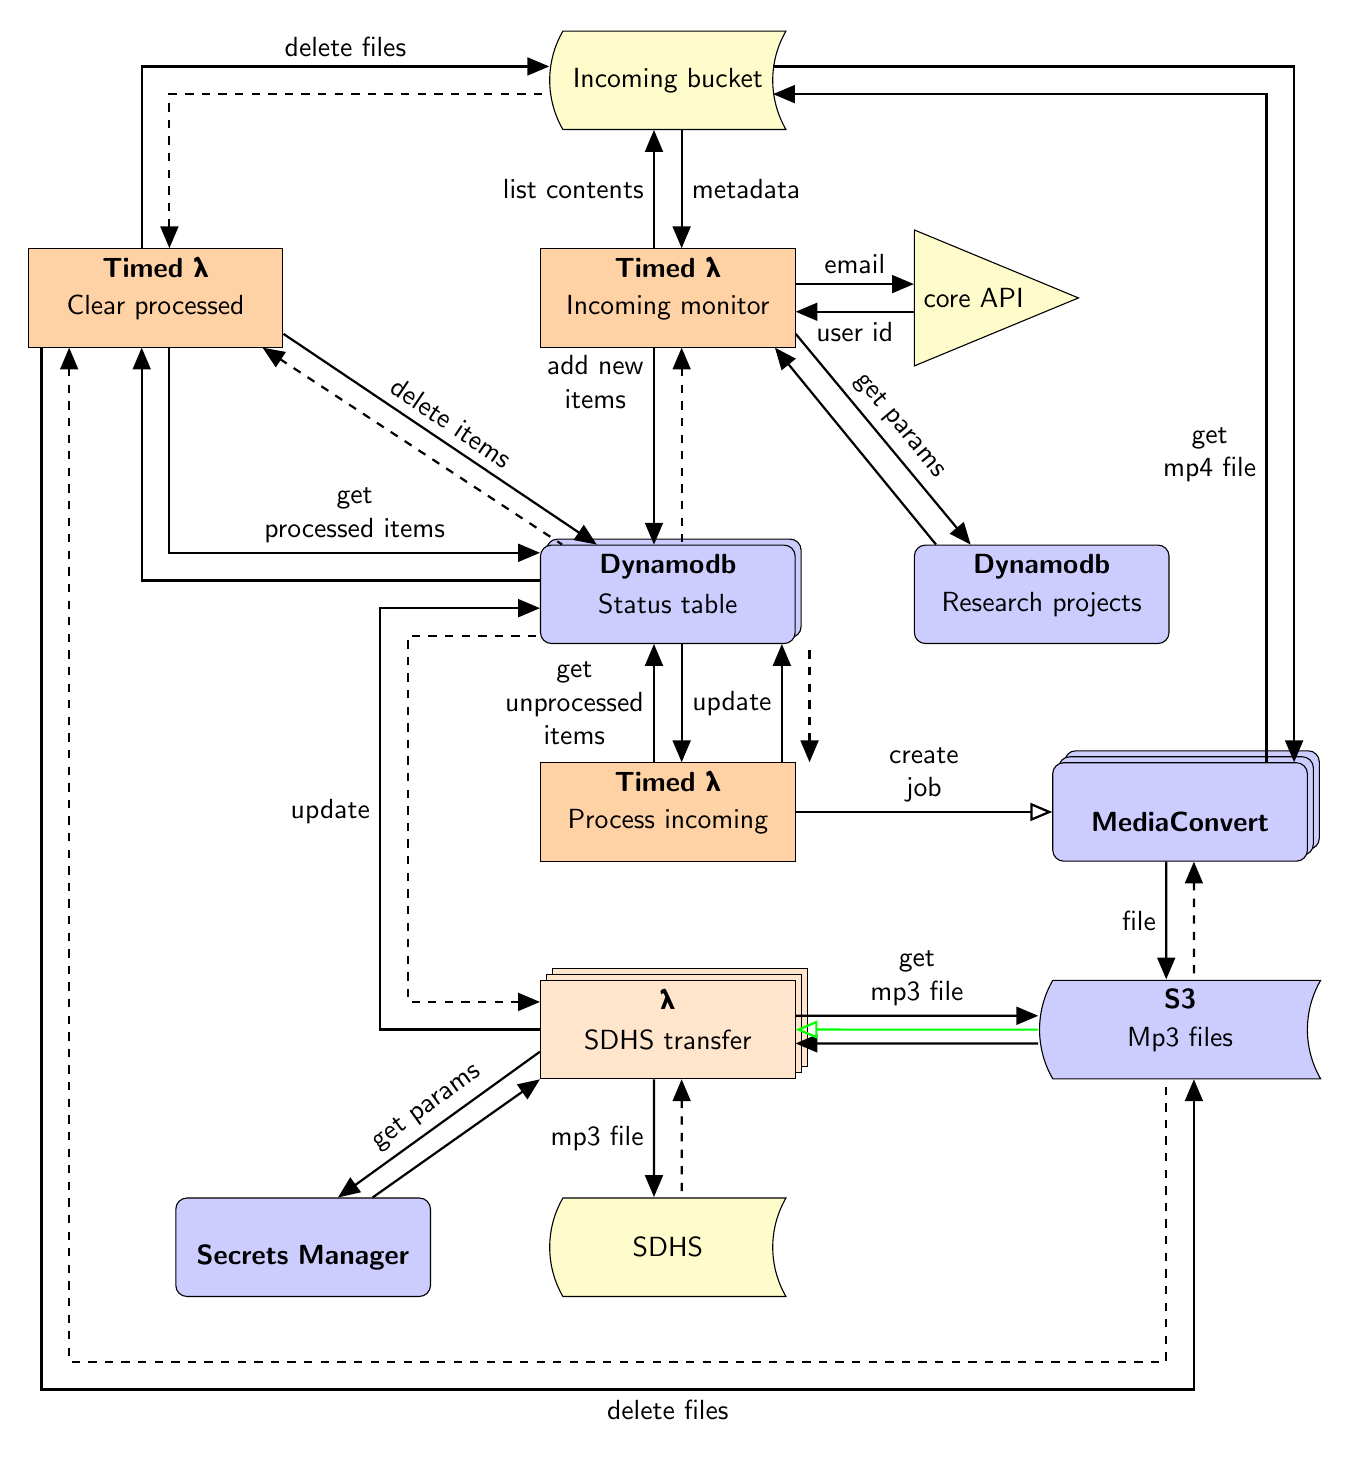
\begin{tikzpicture}[node distance=1.5cm, font={\sf}, align=center]
	%% monitoring
	\node (incoming) [ext-storage] {Incoming bucket};
	\node (monitor) [timed-lambda, below=of incoming] {Incoming monitor};
		\returncall{monitor}{incoming.south}{list contents}{metadata}{vertical}
	\node (core-api) [ext-resource, right=of monitor] {core API};
		\returncall{monitor}{core-api.west}{email}{user id}{}
	
	%% status table
	\node (status-table) [resource, copy shadow, below=of monitor, label={[below]90: \textbf{Dynamodb}}, yshift=-1cm] {Status table};
		\draw [sync, ->, transform canvas={xshift=-0.5em}] (monitor) -- node[anchor=south east, yshift=1em] {add new\\ items} (status-table);
		\draw [sync, <-, transform canvas={xshift=0.5em}, dashed] (monitor) -- (status-table);
	
	%% research projects table
	\node (projects-table) [resource, right=of status-table, label={[below]90: \textbf{Dynamodb}}] {Research projects};
		\draw [sync, ->] ($(monitor.south east) + (0, 0.5em)$) -- node[above, sloped]{get params} (projects-table.145);
		\draw [sync, <-] ($(monitor.south east) - (0.75em, 0)$) -- ($(projects-table.145) - (1.25em, 0)$);
	
	%% Process incoming
	\node (transfer-manager) [timed-lambda, below=of status-table] {Process incoming}; 
		\handshake{transfer-manager.north east}{status-table.south east}{update}{}{vertical}
		\returncall{transfer-manager}{status-table}{get\\ unprocessed\\ items}{}{vertical}
	
	%% MediaConvert
	\node (extract-audio) [resource, double copy shadow, right=of transfer-manager, xshift=5em] {\textbf{MediaConvert}};
		\draw [async, ->] (transfer-manager) -- node[anchor=south] {create\\ job} (extract-audio);
		% incoming
		\draw [sync, ->] ($(extract-audio.north east) + (-1.5em, 0)$) |- node[pos=0.23, anchor=east]{get\\ mp4 file} ($(incoming.east) - (0, 0.5em)$);	
		\draw [sync, <-] ($(extract-audio.north east) + (-0.5em, 0)$) |- ($(incoming.east) + (0, 0.5em)$);	
		% status-table
% 		\draw [sync, ->] ($(extract-audio.north) + (0, 0)$) |- node[pos=0.35, anchor=east]{update} ($(status-table.east) - (0, 0.5em)$);
% 		\draw [sync, <-, dashed] ($(extract-audio.north) + (1em, 0)$) |- ($(status-table.east) + (0, 0.5em)$);	

	%% SDHS transfer
	\node (sdhs-transfer) [lambda, double copy shadow, below=of transfer-manager] {SDHS transfer};
		\coordinate (A) at ($(transfer-manager.west) - (1.5cm,0)$);  
		\draw [sync, ->] ($(sdhs-transfer.west) - (0, 0)$) -| ($(A) - (1.5em,0)$) |- node[pos=0, anchor=east]{update} ($(status-table.west) - (0, 0.5em)$);
		\draw [sync, <-, dashed] ($(sdhs-transfer.west) + (0, 1em)$) -| ($(A) - (0.5em,0)$) |- ($(status-table.west) - (0, 1.5em)$);
		
	%% SDHS
	\node (sdhs) [ext-storage, below=of sdhs-transfer] {SDHS};
		\handshake{sdhs-transfer}{sdhs}{mp3 file}{}{vertical}
	
		%% SecretsManager
	\node (secrets-manager) [resource, left=of sdhs] {\textbf{Secrets Manager}};
		\draw [sync, ->] ($(sdhs-transfer.south west) + (0, 1em)$) -- node[above, sloped]{get params} (secrets-manager.55);
		\draw [sync, <-] ($(sdhs-transfer.south west) - (0, 0)$) -- ($(secrets-manager.55) + (1.25em, 0)$);
		
	
	%% MP3 files
	\node (audio-bucket) [bucket, below=of extract-audio] {Mp3 files};
% 		\draw [async, ->] (transfer-manager.south) -- node[anchor=east]{mp3 metadata} (sdhs-transfer);
		\handshake{extract-audio}{audio-bucket}{file}{}{vertical}
		\returncall{sdhs-transfer}{audio-bucket}{get\\ mp3 file}{}{}	
		\draw[trigger, ->](audio-bucket)--(sdhs-transfer);
		
	%% clearing
	\node (clear-processed) [timed-lambda, left=of monitor, xshift=-5em] {Clear processed};
		\draw [sync, ->] ($(clear-processed.south east) + (0, 0.5em)$) -- node[above, sloped]{delete items} (status-table.145);
		\draw [sync, <-, dashed] ($(clear-processed.south east) - (0.75em, 0)$) -- ($(status-table.145) - (1.25em, 0)$);
		
		\draw [sync, ->] ($(clear-processed.north) - (0.5em, 0)$) |- node[pos=0.75, anchor=south]{delete files} ($(incoming.west) + (0,0.5em)$);
		\draw [sync, <-, dashed] ($(clear-processed.north) + (0.5em, 0)$) |- ($(incoming.west) - (0,0.5em)$);

		\draw [sync, <-] ($(clear-processed.south) - (0.5em, 0)$) |-  ($(status-table.west) + (0,0.5em)$);
		\draw [sync, ->] ($(clear-processed.south) + (0.5em, 0)$) |- node[pos=0.75, anchor=south]{get\\ processed items} ($(status-table.west) + (0,1.5em)$);
	
		\coordinate (B) at ($(sdhs.south) - (0,1cm)$);
		\draw [sync, ->] ($(clear-processed.south west) + (0.5em, 0)$) |- ($(B) - (0,0.5em)$) -| node[pos=0, anchor=north]{delete files} ($(audio-bucket.south) + (0.5em, 0)$);
		\draw [sync, <-, dashed] ($(clear-processed.south west) + (1.5em, 0)$) |- ($(B) + (0,0.5em)$) -| ($(audio-bucket.south) - (0.5em, 0)$);	
	
\end{tikzpicture}
\caption{Thiscovery interview transfer service architecture.}
\end{figure}
\end{center}


\subsection{General}
If several files are added to Incoming bucket at once, they will be processed simultaneously by MediaConvert, which will then trigger simultaneous connections and transfer attempts to the SFTP servers. If this proves problematic, adjust Process incoming to only create one or a few MediaConvert jobs per timed invocation.

\subsection{Specific resources}
\subsubsection{Incoming bucket}
This bucket is not part of the stack. The stack also includes a mock incoming bucket (not represented), which is part of the stack.
\subsubsection{Incoming monitor function}
Calculates and stores in Dynamodb the name that will be used to rename each incoming file at the SFTP server. At present, metadata provided by MyInterview does not contain any project identifier, so the name of the file can only reflect the relationship with the thiscovery user.

Raises error if:
\begin{compactenum}
\item core API does not return user id
\end{compactenum}

%\subsection*{Clear processed function}
%A second call to delete old items from Status table could be included.

\subsubsection*{Status table}
The stack also includes a second table with the same data fields as this one (not represented), which will keep historical transactions for audit purposes. That is, old items will be deleted from the Status table, but a copy of those old items will be stored in this second table.

Each item in Status table relates to a file uploaded to the Incoming bucket by MyInterview. Files created by function Extract audio will not be entered as a separate item in this table.

Each item should include:
\begin{compactenum}
\item \emph{processing status}: new, audio extracted, processed
\item \emph{extraction attempts}: a counter to keep track of failed attempts to run Extract audio on this item
\item \emph{transfer attempts}: a counter to keep track of failed attempts to transfer this item to SDHS
\item \emph{target basename}: calculated basename to use when renaming the original files
\end{compactenum}

\section{Participant info transfer service}\tikzumlset{fill object=black!10, fill call=black!10}
\begin{figure}[h]
\begin{center}
\begin{tikzpicture}
\begin{umlseqdiag}
    \umlbasicobject{s3-to-sdhs}
    \umlbasicobject{thiscovery-core}
    \umlbasicobject{thiscovery-interviews}
    \umlbasicobject{SDHS}
    \begin{umlcallself}[op=get active projects]{s3-to-sdhs}\end{umlcallself}
    \begin{umlcall}[op=project\_id, return=project users, padding=3]{s3-to-sdhs}{thiscovery-core}\end{umlcall}
    \begin{umlfragment}[type=v2]
        \begin{umlcall}[dt=10, op=get future appointments, return=appointment info, padding=3]{s3-to-sdhs}{thiscovery-interviews}\end{umlcall}
%         \begin{umlcallself}[op=store appointment info per user]{s3-to-sdhs}\end{umlcallself}
    \end{umlfragment}
    \begin{umlcall}[op=upload csv, dt=8]{s3-to-sdhs}{SDHS}\end{umlcall}    
\end{umlseqdiag}
\end{tikzpicture}
\caption{Sequence diagram of the thiscovery participant info transfer service.}
\end{center}
\end{figure}


\subsection{General}
Version 2 of the participant info transfer service output should include details of the scheduled interview:
\begin{itemize}
 \item interview datetime
 \item appointment type (usually a proxy for participant group)
 \item Acuity calendar name (proxy for interviewer first name)
\end{itemize}

Version 2 will require:
\begin{compactenum}
 \item a new API endpoint in thiscovery-interviews to retrieve future appoitments
%  \item a new Dynamodb table in s3-to-sdhs to store appointment info indexed by project\_id (hash key), participant id (sort key)
\end{compactenum}

\end{document}
